\documentclass{article}
\usepackage[utf8]{inputenc}
\usepackage{caption}
\usepackage{xcolor}
\usepackage{subfigure}
\usepackage{float}
\usepackage{natbib}
\usepackage{graphicx}
\usepackage{csvsimple}
\usepackage[export]{adjustbox}

\begin{document}


\begin{titlepage}
	\centering 
	\scshape
	\vspace*{\baselineskip}
	\rule{\textwidth}{1.6pt}\vspace*{-\baselineskip}\vspace*{2pt}
	\rule{\textwidth}{0.4pt} 
	\vspace{0.75\baselineskip}
	
	{\Large CS 374 : Computational and Numerical Methods \\\vspace{0.75\baselineskip} Set 7}
	\vspace{0.75\baselineskip}
	
	\rule{\textwidth}{0.4pt}\vspace*{-\baselineskip}\vspace{3.2pt} 
	\rule{\textwidth}{1.6pt}
	
	\vspace{2\baselineskip}  
	The Bisection Method
	
	\vspace*{3\baselineskip}
	
	\vspace{0.5\baselineskip} %originally 0.5
	
	{\scshape\large Purvil Mehta (201701073) \\ Bhargey Mehta (201701074) \\} 
	
	\vspace{1\baselineskip} 
	
	\textit{Dhirubhai Ambani Institute of Information and Communication Technology \\ Gandhinagar\\} 
	\vspace*{2\baselineskip}
	\today


\end{titlepage}

\newpage
\tableofcontents
\newpage
\section{Question-1}
\subsection{Plots}
\begin{figure}[!h]
\centering
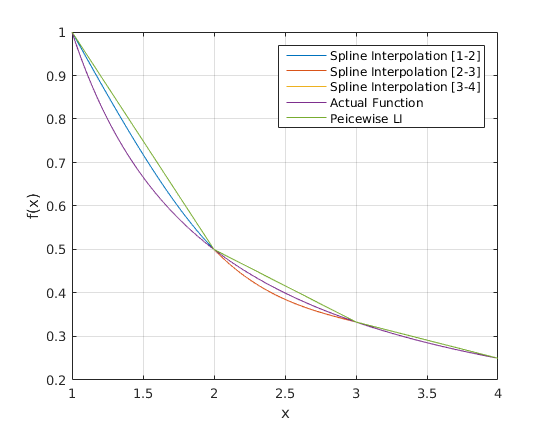
\includegraphics[scale = 0.6]{7_1_a.png}
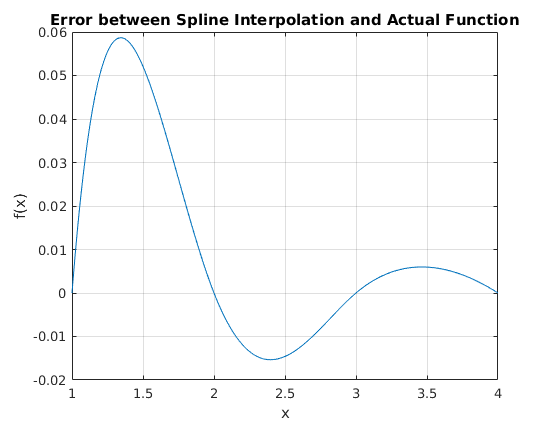
\includegraphics[scale = 0.6]{7_1_b.png}
\caption{Comparison of Linear Piece wise, Spline and Actual function and it's Error}
\end{figure}
\newpage

\section{Question-2}
\subsection{Plots}
\begin{figure}[!h]
\centering
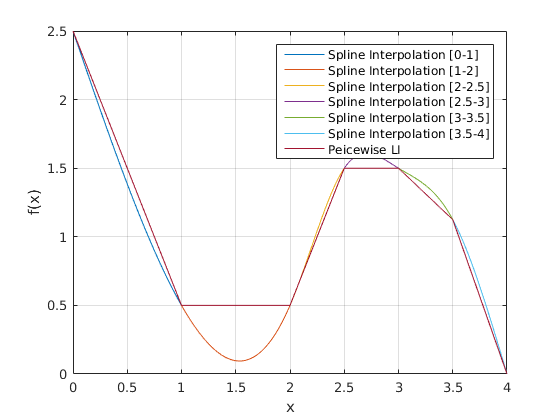
\includegraphics[scale=0.8]{7_2.png}
\caption{Comparison of Linear Piece-wise and Spline}
\end{figure}
\newpage

\section{Question-3}
\subsection{Plots}
\begin{figure}[!h]
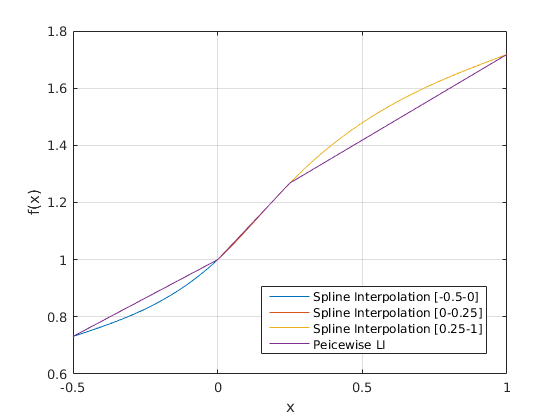
\includegraphics[scale=0.5]{7_3_a.png}
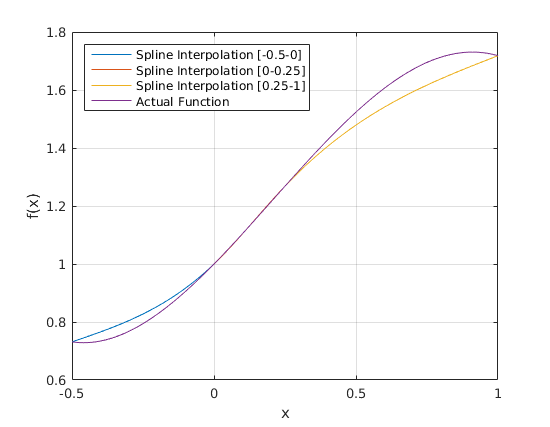
\includegraphics[scale=0.5]{7_3_b.png}
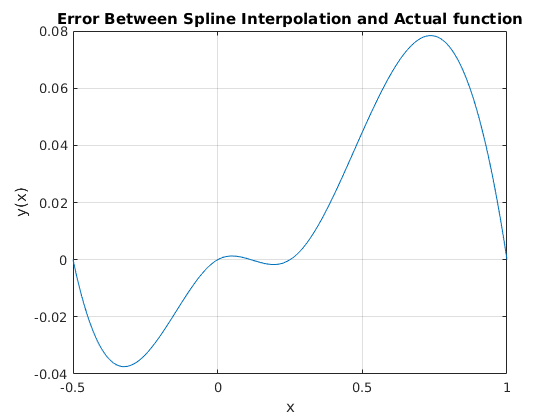
\includegraphics[scale=0.6]{7_3_c.png}
\caption{Comparison of Linear Piece-wise and Spline Interpolation and It's Error}
\end{figure}
\newpage

\section{Question-4}
\subsection{a}
\subsubsection{Equations}
$$
s(x) = \left\{
        \begin{array}{ll}
            x^{3} - x + 1 & x\in [0,1]\\
            - x^{3} + 6 x^{2} - 7 x + 3 & x\in [1,2]
        \end{array}
    \right.
$$

\subsubsection{Plots}
\begin{figure}[H]
\centering
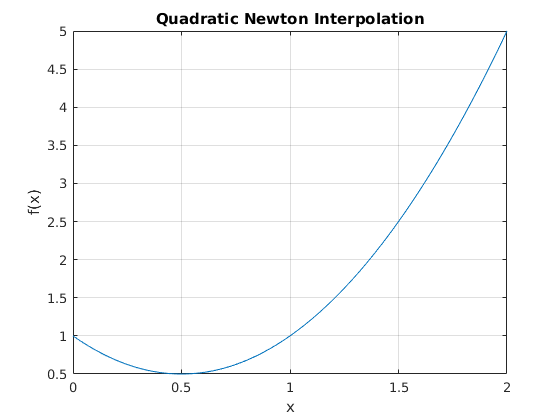
\includegraphics[scale=0.55]{7_4_1_a.png}
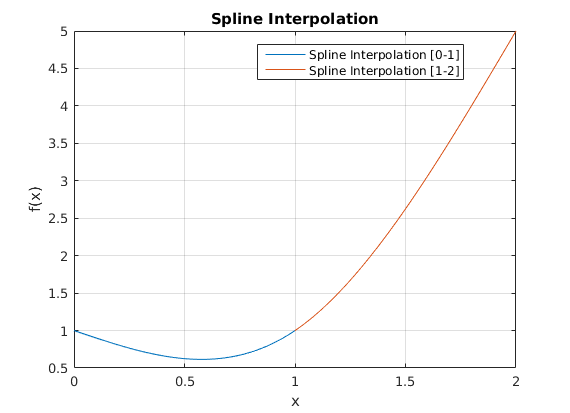
\includegraphics[scale=0.55]{7_4_1_b.png}
\caption{}
\end{figure}
\newpage
\subsection{b}
\subsubsection{Equations}
$$
s(x) = \left\{
        \begin{array}{ll}
            \frac{47 x^{3}}{56} + \frac{411 x^{2}}{56} - \frac{79 x}{4} + \frac{125}{7} & \quad x \in [1,2] \\
            \frac{47 x^{3}}{56} + \frac{411 x^{2}}{56} - \frac{79 x}{4} + \frac{125}{7} & \quad x \in [2,3] \\
            \frac{23 x^{3}}{56} + \frac{195 x^{2}}{56} - \frac{229 x}{28} + \frac{44}{7} & x\in [3,4]\\
            \frac{27 x^{3}}{56} - \frac{405 x^{2}}{56} + \frac{971 x}{28} - \frac{356}{7} & x\in [4,5]
        \end{array}
    \right.
$$

\subsubsection{Plots}
\begin{figure}[H]
\centering
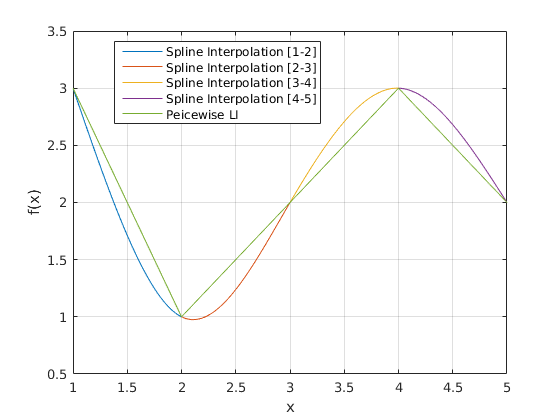
\includegraphics[scale=0.8]{7_4_2.png}
\caption{}
\end{figure}

\newpage
\subsection{c}
\subsubsection{Equations}
$$
s(x) = \left\{
        \begin{array}{ll}
            1.81 x^{3} + 0.047 x & \quad x \in [0,0.5] \\
            - 5.048 x^{3} + 10.3 x^{2} - 5.1 x + 0.85 & \quad x \in [0.5,1] \\
            2.52 x^{3} - 12.43 x^{2} + 17.62 x - 6.71 & \quad x\in [1,2]\\
            - 0.91 x^{3} + 8.14 x^{2} - 23.52 x + 20.71 & \quad x\in [2,3]
        \end{array}
    \right.
$$

\subsubsection{Plots}
\begin{figure}[H]
\centering
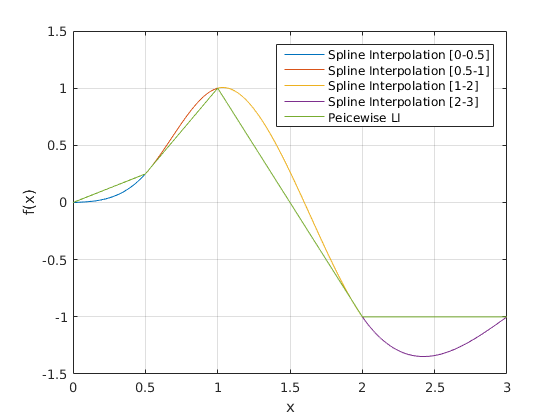
\includegraphics[scale=0.8]{7_4_3.png}
\caption{}
\end{figure}

\newpage
\subsection{d}
\subsubsection{Equations}
$$
s(x) = \left\{
        \begin{array}{ll}
            0.45 x^{3} - 1.25 x + 1.4 & \quad x \in [0,1] \\
            - 1.03 x^{3} + 4.44 x^{2} - 5.68 x + 2.89 & \quad x\in [1,2]\\
            2.02 x^{3} - 13.85 x^{2} + 30.91 x - 21.51 & \quad x \in [2,2.5] \\
            - 0.65 x^{3} + 6.16 x^{2} - 19.14 x + 20.19 & \quad x\in [2.5,3] \\
            - 0.096 x^{3} + 1.16 x^{2} - 4.12 x + 5.18 & \quad x\in [3,4] 
        \end{array}
    \right.
$$

\subsubsection{Plots}
\begin{figure}[H]
\centering
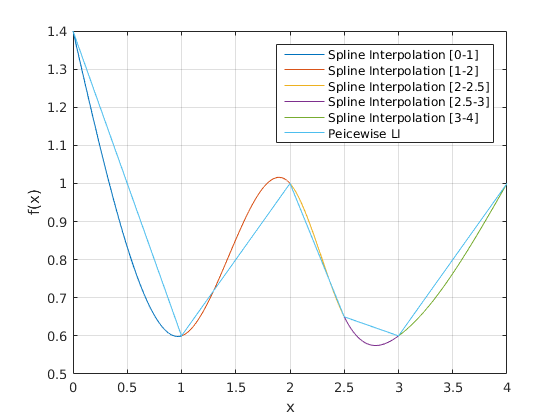
\includegraphics[scale=0.8]{7_4_4.png}
\caption{}
\end{figure}

\end{document}